\documentclass{article}

\usepackage{amsmath}
\usepackage{bm}
\usepackage{caption}
\usepackage{subcaption}
\usepackage{enumerate}
\usepackage{float}
\usepackage{mathtools}
\usepackage[section]{placeins}
\usepackage{url}
\usepackage[ruled]{algorithm2e}
\usepackage{hyperref}
\usepackage{color}
\usepackage[a4paper, total={7in, 11in}]{geometry}
\usepackage{amssymb}
\usepackage{color}
\usepackage{enumitem,xcolor}
\usepackage[normalem]{ulem}
\usepackage[ruled]{algorithm2e}
\usepackage{tikz}
\usetikzlibrary{fit,positioning}


\title{Genre-topic model for meaning change}
\author{Valerio Perrone}



\begin{document}
\maketitle 

\section{The model}
We extend the model proposed by Lea to include genre meta-data. This is inspired by the author-topic model\footnote{ \url{https://mimno.infosci.cornell.edu/info6150/readings/398.pdf}}. In this setting, instead of having a single probability distribution over meanings at each time, we have $G$ different probability distributions, one for each genre. This makes it possible to leverage available genre information to improve inference and answer a set of additional research questions. For instance, we can find the genre most likely associated to a meaning, the most unusual meaning for genre, and which genres have the most similar meanings.


\begin{algorithm}
\caption{Generative model}
\label{algo2}
\SetAlgoLined

Draw $K^\phi \sim Gamma(a,b)$; \\
\For{\text{time} $t = 1,\dots,T$}{

	\For{genre $g = 1,\dots,G$}{
		Draw sense distribution $\phi^t_g \mid \phi^{-t}_g, K^\phi  \sim N( \frac{1}{2}(\phi^{t-1} + \phi^{t+1}), K^\phi)$
	}
	
	\For{sense $k = 1,\dots,K$}{
		Draw word distribution $\psi^t_g \mid \psi^{-t}_g, K^\psi  \sim N( \frac{1}{2}(\psi^{t-1} + \psi^{t+1}), K^\psi)$ \\
		
	}
	\For{document $d = 1,\dots,D$}{
	Draw genre $x^d \sim U(\{ g_1, \dots, g_G \} )$; \\ %Note: this is observed. no need to sample it.
	Draw sense $z^d \mid x^d \sim \text{Mult}(\phi^t_g)$; \\
	
		\For{context position $i = 1,\dots,I$}{
		Draw word $w^{d,i} \sim \text{Mult}(\psi^{t,z^d})$; \\
		}
	}
}

\end{algorithm}



\section{Marginal graphical model at each time $t$}

\begin{figure}[h!]
\centering
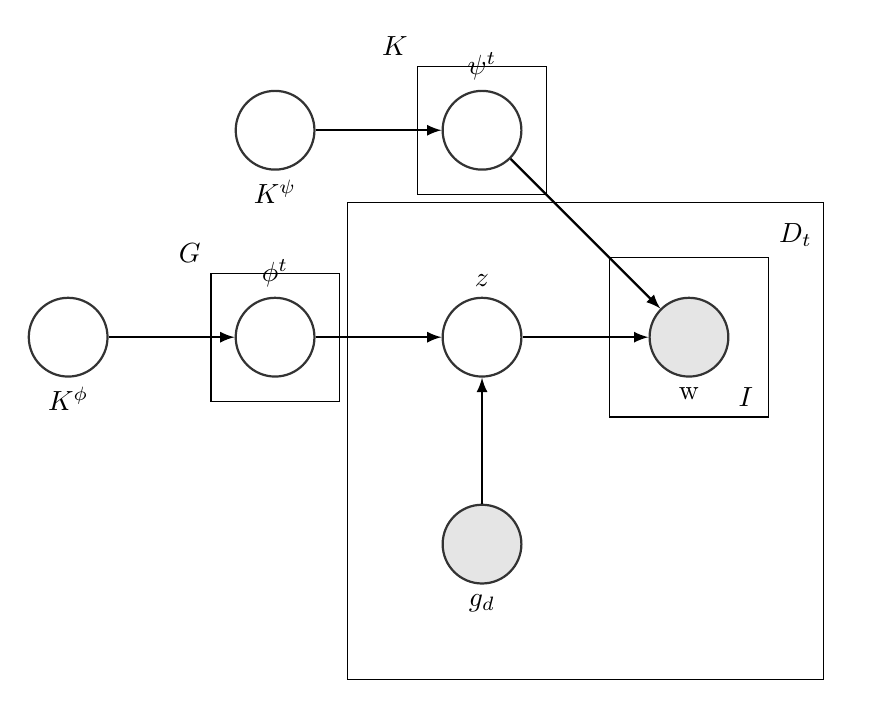
\begin{tikzpicture}
\tikzstyle{main}=[circle, minimum size = 10mm, thick, draw =black!80, node distance = 16mm]
\tikzstyle{connect}=[-latex, thick]
\tikzstyle{box}=[rectangle, draw=black!100]
  \node[main, fill = white!100] (alpha) [label=below:$K^\phi$] { };
  \node[main] (theta) [right=of alpha,label=above:$\phi^t$] { };
  \node[main] (z) [right=of theta,label=above:$z$] {};
  \node[main] (psi) [above=of z,label=above:$\psi^t$] { };
  \node[main, fill = white!100] (kappa) [left=of psi, label=below:$K^\psi$] { };
  \node[main, fill = black!10] (genre) [below=of z,label=below:$g_d$] { };
  \node[main, fill = black!10] (w) [right=of z,label=below:w] { };
  \path (alpha) edge [connect] (theta)
        (theta) edge [connect] (z)
		(z) edge [connect] (w)
		(kappa) edge [connect] (psi)
		(psi) edge [connect] (w)
		(genre) edge [connect] (z);
  \node[rectangle, inner sep=0mm, fit= (z) (w),label=below right:$I$, xshift=13mm] {};
   \node[rectangle, inner sep=5mm,draw=black!100, fit= (w), label=above right:$D_t$, , xshift=0mm] {};
  \node[rectangle, inner sep=12mm,draw=black!100, fit= (genre) (w)] {};
   \node[rectangle, inner sep=3mm,draw=black!100, fit= (theta), label=above left:$G$,] {};
      \node[rectangle, inner sep=3mm,draw=black!100, fit= (psi), label=above left:$K$,] {};
  \node[rectangle, inner sep=4.6mm, fit= (z) (w),xshift=12.5mm] {};
\end{tikzpicture}
\end{figure}


\section{Inference}
Lea's inference with the following adaptations:
\begin{itemize}
\item Sample the distribution over senses \textit{for each genre $g=1,\dots,G$}
\item Sample the sense assignments conditioned on the observed genre:
\begin{align*}
p(z^d \mid g^d, \textbf{w}, t, \phi, \psi) 
&\propto  p(z^d \mid g^d, t) p( \textbf{w} \mid t, z^d) \\
& \phi^t_{g} \prod_{w \in \textbf{w}} \psi^{t,z^d}_w
\end{align*}

\end{itemize}

\textbf{Note}: inference is simpler than in the author-topic model. In that case, while the authors are observed, they still need to sample to author assignment for each word. In our case, we observe one genre and assume all words come from that genre, hence we have no genre assignment to sample.




\end{document}\grid
\grid
\grid
\grid
